\subsection{Categorical target features}

We're gonna start with a \textbf{boolean target}, for which we already mentioned the \textbf{confusion matrix} before, but gonna go into more detail now.

\begin{figure}[H]
  \centering
  \begin{subfigure}{0.4\textwidth}
    \centering
    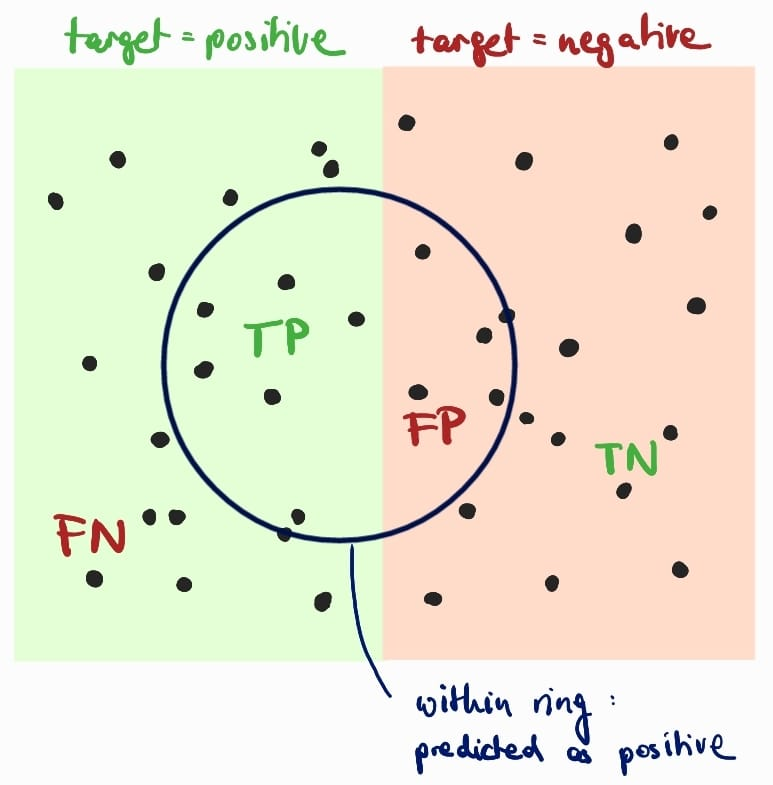
\includegraphics[width=\textwidth]{assets/sl/ct__confusion.jpg}
  \end{subfigure}

  \caption{Confusion matrix visualized on dataset}
  \label{fig:7_confusion_matrix}
\end{figure}

With $TP$, $FP$, $FN$, and $TN$ we cam make some further definitions:
\begin{itemize}
  \item $FP$ is also known as \textbf{type I error}\sidenote{Type I error}, or false alarms
  \item $FN$ is also known as \textbf{type II error}\sidenote{Type II error}, or missed alarms
  \item Further we have some rates:
  \begin{align*}
    \text{True positive rate}: TPR\sidenote{$TPR$} &= \frac{\scriptstyle TP}{\scriptstyle TP+FN} = 1-FNR
      &&\begin{array}{l}\text{\color{gray}\footnotesize fraction of positives}\\\text{\color{gray}\footnotesize classified as positive}\end{array}\\
    \text{True negative rate}: TNR\sidenote{$TNR$} &= \frac{\scriptstyle TN}{\scriptstyle TN+FP} = 1-FPR
      &&\begin{array}{l}\text{\color{gray}\footnotesize fraction of negatives}\\\text{\color{gray}\footnotesize classified as negative}\end{array}\\
    \text{False negative rate}: FNR\sidenote{$FNR$} &= \frac{\scriptstyle FN}{\scriptstyle FN+TP} 
      &&\begin{array}{l}\text{\color{gray}\footnotesize fraction of positives}\\\text{\color{gray}\footnotesize classified as negative}\end{array}\\
    \text{False positive rate}: FPR\sidenote{$FPR$} &= \frac{\scriptstyle FP}{\scriptstyle FP+TN} 
      &&\begin{array}{l}\text{\color{gray}\footnotesize fraction of negatives}\\\text{\color{gray}\footnotesize classified as positive}\end{array}\\
  \end{align*}
  \item Further, we define:
  \begin{align*}
    \text{Accuracy}\sidenote{Accuracy}: ACC &= \frac{\scriptstyle TP+TN}{\scriptstyle TP+TN+FP+FN}
      &&\begin{array}{l}\text{\footnotesize Missclassifications}:\\ \scriptstyle 1-ACC\end{array}\\
    \text{Precision}\sidenote{Precision}: precision &= \frac{\scriptstyle TP}{\scriptstyle TP+FP}
      &&\begin{array}{l}\text{\color{gray}\footnotesize within circle,}\\\text{\color{gray}\footnotesize fraction of }\scriptstyle TP\end{array}\\
    \text{Recall}\sidenote{Recall}: recall &= \frac{\scriptstyle TP}{\scriptstyle TP+FN} = TPR
      &&\begin{array}{l}\text{\color{gray}\footnotesize green part,}\\\text{\color{gray}\footnotesize fraction of }\scriptstyle TP\end{array}\\
    F_1\text{-measure}\sidenote{$F_1$-measure}: F_1 &= 2\frac{\scriptstyle prec \cdot recall}{\scriptstyle prec + recall} = \frac{\scriptstyle TP}{\scriptstyle TP+\frac{1}{2}(FP+FN)}
      &&\begin{array}{l}\text{\color{gray}\footnotesize harmonic mean of}\\\text{\color{gray}\footnotesize precision and recall}\end{array}\\\\
    \text{Sensitivity}\sidenote{Sensitivity}: sensitivity &= \frac{\scriptstyle TP}{\scriptstyle TP+FN} = TPR = recall\\
    \text{Specificity}\sidenote{Specificity}: specificity &= \frac{\scriptstyle TN}{\scriptstyle TN+FP} = TNR
      &&\begin{array}{l}\text{\color{gray}\footnotesize red part,}\\\text{\color{gray}\footnotesize fraction of }\scriptstyle TN\end{array}
  \end{align*}
\end{itemize}

With these measures, we can now evaluate the data. Consider e.g. \textbf{imbalanced data} where we have:
\begin{itemize}
  \item $99\%$ in a dataset of size $100$ is positive ($\rightarrow$ $99$ instances positive, $1$ negative)
  \item Our classification always predicts a positive label
  \item We then have:
  \begin{align*}
    precision &= \frac{99}{99+1} = 0.99& recall&=\frac{99}{99+0} = 1
  \end{align*}
  \item When we now apply simple average class accuracy, where each class has the same weight independent of size, we get the following value:
  \begin{align*}
    average\ class\ ACC & = \frac{1}{|classes|}\sum_{c\in classes} recall_c\\
    &= \frac{1}{2}\left(\frac{99}{99+0} + \frac{0}{0+1}\right)  = 0.5
  \end{align*}
  \item When we instead use a \textbf{harmonic mean}, again with each class having the same weight independent of size, we get:
  \begin{align*}
    average\ class\ ACC_{HM} & = \frac{1}{\frac{1}{|classes|}\sum_{c\in classes} \frac{1}{recall_c}}\\
    &= \left(\frac{1}{2}\left(\frac{99+0}{99} + \frac{0+1}{0}\right)\right)^{-1}  = "0.0"
  \end{align*}
\end{itemize}

\begin{figure}[H]
  \centering
  \begin{subfigure}{0.8\textwidth}
    \centering
    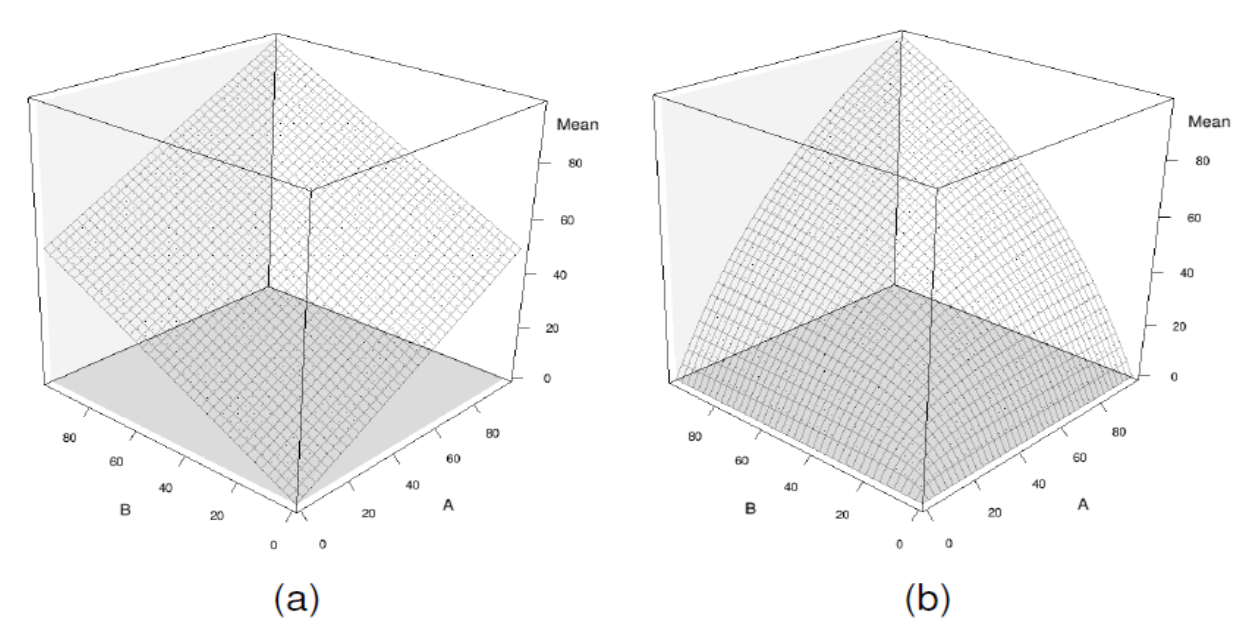
\includegraphics[width=0.8\textwidth]{assets/sl/ct__harmonic_mean.png}

    \text{\footnotesize For HM (visualized in b), both A and B need to be good for the HM to be good}
  \end{subfigure}

  \caption{Arithmetic and harmonic mean}
  \label{fig:7_ct_harmonic_mean}
\end{figure}

We can not only use the confusion matrix by itself but also weigh or quantify good and bad. This is then the \textbf{profit matrix}\sidenote{Profit matrix}.
\begin{itemize}
  \item We then have the entries $TP_{profit}$, $FP_{profit}$, $FN_{profit}$, and $TN_{profit}$
  \item By adding a profit quantification, we can express that $FP$ and $FN$ don't always have the same costs (e.g. car accident)
\end{itemize}

\begin{figure}[H]
  \centering
  \begin{subfigure}{0.7\textwidth}
    \centering
    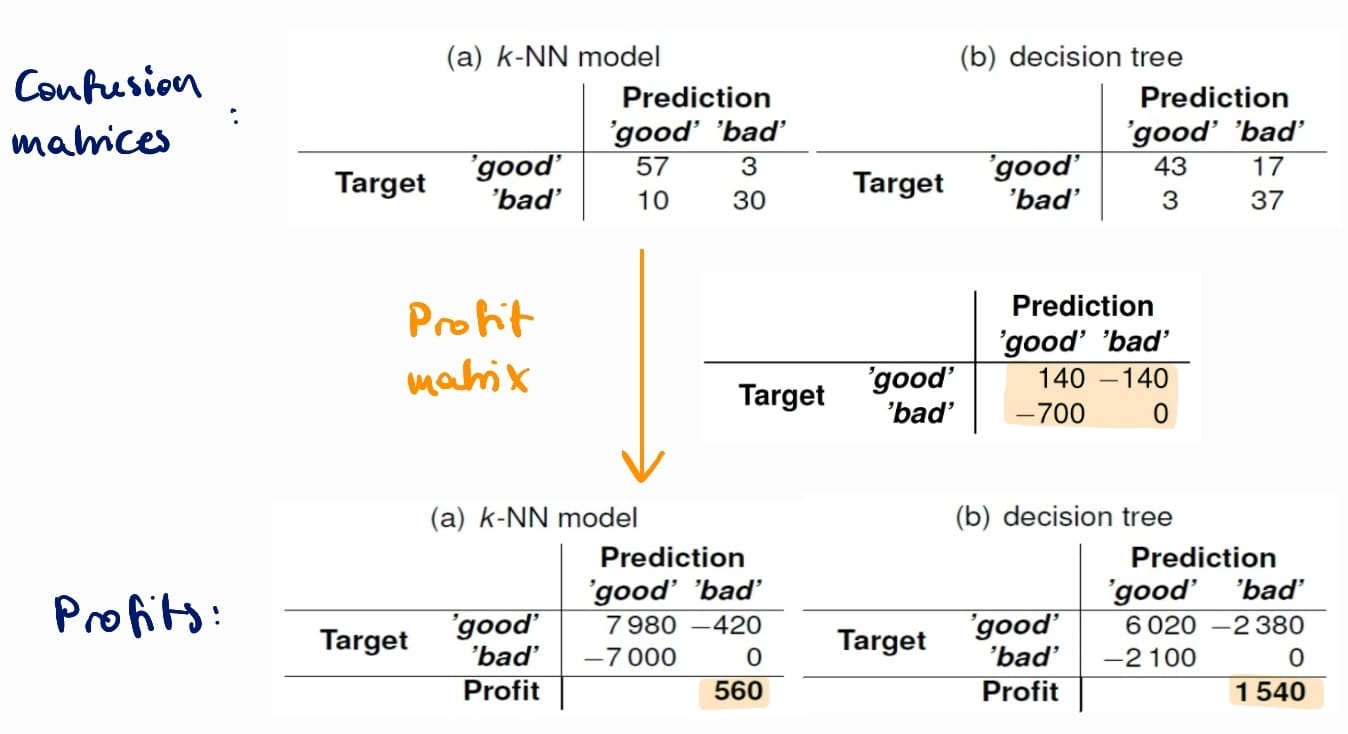
\includegraphics[width=\textwidth]{assets/sl/ct__profit.jpg}
  \end{subfigure}

  \caption{Profit matrix principle}
  \label{fig:7_ct_profit}
\end{figure}
